\documentclass{beamer}
\setbeamertemplate{navigation symbols}{}
%%%%%%%%%%%%%%%%%%%%%%%%%%%%%%%%%%%%%%%command added by me
\usepackage{array}
\usepackage{tabularx}
\usepackage{multirow} 
\usepackage{graphicx}
\usepackage{multirow}
%\usepackage{subfig}

%%%%%%%%%%%%%%%%%%%%%%%%%%%%%%%%%%%%%%%%%%%%%%%%%%%%%%%%%%%%%%%%%%%%%
\usetheme{Madrid}%
%\usetheme{Boadilla}
%\usetheme{Singapore}
%\usetheme{Warsaw}
%\usetheme{Dresden}
%\usetheme{Berlin}
%\usetheme{Bergen}
%\usetheme{Boadilla}
%\usetheme{Copenhagen}
%\usetheme{Hannover}
%\usetheme{Luebeck}
%\usetheme{Marburg}
%\usetheme{Pittsburgh}
%\usetheme{default}
%\usetheme{Singapore}
%\usetheme{boxes}

%\usecolortheme{beaver}
%%%%%%%%%%%%%%%%%%%%%%%%%%%%%%%%%%%%%%%%%%%%%%%%%%%%%%%%%%%%%%%%%%%%%
%\beamersetuncovermixins{\opaqueness<1>{25}}{\opaqueness<2->{15}}
\begin{document}

\title[SSC 2014]{Partial Stratification in Two-Sample Capture-Recapture Experiments}  
\author[Lasantha Premarathna]{Lasantha Premarathna}
\institute[SFU]{Department of Statistics and Actuarial Science, \\ Simon Fraser University, \\ Burnaby, BC.}
\date{May 24, 2014} %{\today}

%%%%%%%%%%%%%%%%%%%%%%%%%%%%%%%%%%%%%%%%%%%%%%%%%%%%%%%%%%%%%%%%%%%%%%%%%%%%%%%%%%%%
\begin{frame}
\titlepage
\end{frame}
%%%%%%%%%%%%%%%%%%%%%%%%%%%%%%%%%%%%%%%%%%%%%%%%%%%%%%%%%%%%%%%%%%%%%%%%%%%%%%%%%%%%
\begin{frame}\frametitle{Outline}\tableofcontents
\end{frame} 

%%%%%%%%%%%%%%%%%%%%%%%%%%%%%%%%%%%%%%%%%%%%%%%%%%%%%%%%%%%%%%%%%%%%%%%%%%%%%%%%%%%%
\section{Introduction} 
\begin{frame}\frametitle{Introduction} %\[allowframebreaks]{Introduction} 
{\scriptsize 
\begin{itemize}
\item \textbf{Capture-recapture Method}

	\begin{itemize}
	\item  {\scriptsize Capture-recapture is a method commonly used in ecology to estimate an animal population size.}
	\end{itemize}
\item \textbf{Lincoln-Petersen Method.}
	\begin{itemize}
	\item {\scriptsize A simple two-sample capture-recapture method}
	\item  {\scriptsize Lincoln-Petersen estimte for population abundance }

	$$\hat{N} = n_{1}n_{2}/m$$

	{\scriptsize where $n_{1}$ is a sample of animals captured, marked and released in the first capture occasion and $n_{2}$ is the total number of animals captured in the second
	occasion and $m$ is the number of marked  animals captured in the second occasion.}
	\end{itemize}
\item \textbf{Partial Stratification}
\begin{itemize}
\item {\scriptsize Animals may vary in capture probability due to sex,size or many other factors. \item Heterogenity in catchability is know to lead bias in two-sample Lincoln-Petersen estimate of population size.}
\item {\scriptsize  stratification adress the capture heterogenity.}
\item {\scriptsize Importance of partial stratification}
\end{itemize}
\end{itemize}

}

\end{frame}

%%%%%%%%%%%%%%%%%%%%%%%%%%%%%%%%%%%%%%%%%%%%%%%%%%%%%%%%%%%%%%%%%%%%%%%%%%%%%%%%%%%%
\section{Model Development}
\subsection{Notation} 
\begin{frame} \frametitle{Model Development}
\textbf{{\footnotesize Notation}}

{\scriptsize Partial Stratification in Two-Sample Capture-Recapture Experiments
\begin{center}
\begin{tabular}{c l}
$T$ & Number of capture occasions,  where $ T = 2$\\
$t$ & index for capture occasion, where $t = 1, T$\\
$s$ & Number of categories\\
$k$ & index for category, where $k = 1,2,...,s$ \\
& \\
$0$ &animal is not captured \\
$U$ &animal is captured but not stratified\\
$C_{k}$ &animal is captured and identified the category $k$\\
\end{tabular}
\end{center}
}

{\scriptsize Sampling protocol}
\begin{figure}[h]
    \centering
    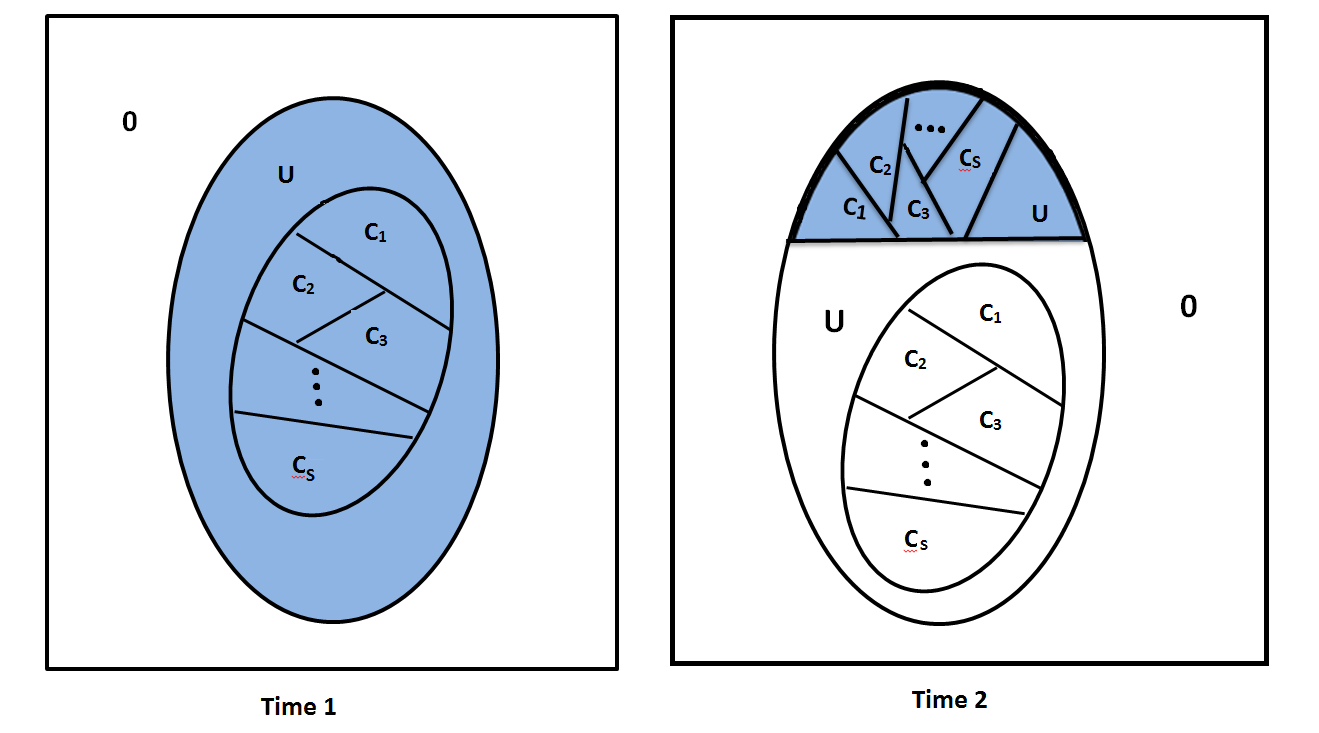
\includegraphics[scale=0.17]{CaptureReCap_General.png}
%    \caption{Partial Stratification in Two Sample Capture Recapture Experiments}
%    \label{fig:PSTSCRE}
\end{figure}
\end{frame}
%%%%%%%%%%%%%%%%%%%%%%%%%%%%%%%%%%%%%%%%%%%%%%%%%%%%%%%%%%%%%%%%%%%%%%%%%%%%%%%%%%%%%
%%%%%%%%%%%%%%%%%%%%%%%%%%%%%%%%%%%%%%%%%%%%%%%%%%%%%%%%%%%%%%%%%%%%%%%%%%%%%%%%%%%%%
\subsection{Assumptions}
\begin{frame} \frametitle{Model Development}
\textbf{{\footnotesize Assumptions}}
{\footnotesize 
\begin{itemize}
 \item The population is \textbf{closed} (geographically and demographically). The number of individuals does not change
 during the study through birth or immigration and/or death or emigration
 \item Mark status is correctly identified at recovery and unique to each animal
 \item Marks are not lost between sampling occasions
 \item Capture and marking does not affect subsequent catchability of an animal
 \item The population can be  divided into non-overlapping categories
 \item Sub-sample at each occasion is a random sample of animals that are not marked
 \item categories of the animals in the sub-sample are successfully identified
 \item Animal captures are independent
 \end{itemize}
}
\end{frame}

%%%%%%%%%%%%%%%%%%%%%%%%%%%%%%%%%%%%%%%%%%%%%%%%%%%%%%%%%%%%%%%%%%%%%%%%%%%%%%%%%%%%%%
%%%%%%%%%%%%%%%%%%%%%%%%%%%%%%%%%%%%%%%%%%%%%%%%%%%%%%%%%%%%%%%%%%%%%%%%%%%%%%%%%%%%%%
\subsection{Capture Histories, Statistics, Parameters}
\begin{frame} \frametitle{Model Development}
\textbf{{\footnotesize Capture Histories}}
\vspace{2pt}

{\scriptsize 
$\qquad U0, UU, 0U, C_{k}0, C_{k}C_{k}, 0C_{k}$ and $00$
\vspace{2pt}

\hspace{1.5cm}- There are $3s + 4$ capture histories
\vspace{2pt}

\hspace{1.5cm}- Capture history $00$ is unobservable
}
\vspace{6pt}

\textbf{{\footnotesize Statistics}}
\vspace{2pt}

{\scriptsize 
$\qquad n_{U0}, n_{UU}, n_{0U}, n_{C_{k}0}, n_{ C_{k}C_{k}},n_{0C_{k}}$  are the number of animals related to the \textit{observable} capture histories
 and $n$ is the number of animals  caught in the study 
 
 $\qquad \qquad \qquad n =n_{U0}+n_{UU}+n_{0U}+  \sum\limits_{k} n_{C_{k}0} +  \sum\limits_{k} n_{ C_{k}C_{k}} +  \sum\limits_{k} 0C_{k}    $
}
\vspace{6pt}

\textbf{{\footnotesize Model Parameters}}
\vspace{2pt}
{\tiny 
\begin{center}
\begin{tabular}{c l}
\vspace{4pt}
$p_{tk}$ &Capture probability of animals belong to category $k$ at sampling occasion $t$\\ \vspace{4pt}
$\lambda_k $ & Proportion of category $k$ animals in the population\\ \vspace{4pt}
$\theta_t$ & sub-sample proportion at sampling occasion $t$\\ \vspace{4pt}
$N$ & Population size 
\end{tabular}
\end{center}
$\qquad \qquad \qquad \qquad \qquad \qquad \qquad \lambda_s  = 1 - \sum\limits_{k=1}^{s-1}\lambda_k $
}
\end{frame}


%%%%%%%%%%%%%%%%%%%%%%%%%%%%%%%%%%%%%%%%%%%%%%%%%%%%%%%%%%%%%%%%%%%%%%%%%%%%%%%%%%%%%%
\begin{frame} \frametitle{Model Development}
\textbf{{\footnotesize Probability Statements of Capture History}}
{\scriptsize  
\begin{center}
\begin{tabular}{l l}
\vspace{4pt}
$P_{U0}$&$= \sum\limits_{k}^{s} \lambda_{k}p_{1k}(1-\theta_{1})(1-p_{2k})  \vspace{4pt}$ \\ \vspace{4pt}
$P_{UU}$&$= \sum\limits_{k}^{s} \lambda_{k}p_{1k}(1-\theta_{1})p_{2k} $\\ \vspace{4pt}
$P_{0U}$&$= \sum\limits_{k}^{s} \lambda_{k}(1-p_{1k})p_{2k} (1-\theta_{2}) $\\ \vspace{4pt}
$P_{C_{k}0}$&$= \lambda_{k}p_{1k}\theta_{1}(1-p_{2k})$\\ \vspace{4pt}
$P_{C_{k}C_{k}}$&$= \lambda_{k}p_{1k}\theta_{1}p_{2k}$\\ \vspace{4pt}
$P_{0C_{k}}$&$= \lambda_{k}(1-p_{1k})p_{2k} \theta_{k}$\\ \vspace{4pt}
$P_{00}$&$= \sum\limits_{k}^{s} \lambda_{k}(1-p_{1k})(1-p_{2k}) $\\ 
\end{tabular}
\end{center}


\begin{itemize}
\item $P_{U0} + P_{UU}+P_{0U} + \sum\limits_{k}P_{C_{k}0} +\sum\limits_{k}P_{0C_{k}} +\sum\limits_{k}P_{0C_{k}} +P_{00} = 1$
\item Even though the capture history $00$ is unobservable, the probability statement cab be  explicitly given
\end{itemize}
}
\end{frame}


%%%%%%%%%%%%%%%%%%%%%%%%%%%%%%%%%%%%%%%%%%%%%%%%%%%%%%%%%%%%%%%%%%%%%%%%%%%%%%%%%%%%%%
\subsection{Likelihood}
\begin{frame} \frametitle{Model Development}
\textbf{{\footnotesize The  Model}}
\vspace{6pt}

{\footnotesize Multinomial distribution with unknown index }
\vspace{6pt}

{\tiny 
 \begin{multline*}
% \begin{split}
f(.) = \frac{N!}{n_{U0}!\quad n_{UU}!\quad n_{0U}! \quad \prod\limits_{k} n_{C_{k}0}! \quad  \prod\limits_{k=1}n_{C_{k}C_{k}}! \quad \prod\limits_{k} n_{0C_{k}}! \quad (N-n)!} \quad \times \\
\qquad \qquad \qquad (P_{U0})^{n_{U0}}(P_{UU})^{n_{UU}}(P_{0U})^{n_{0U}} \quad \times \\
\prod\limits_{k=1}^{s} (P_{C_{k}0})^{n_{C_{k}0}} \quad \times \\
\qquad \prod\limits_{k=1}^{s} (P_{C_{k}C_{k}})^{n_{ C_{k}C_{k}}} \quad \times \\
\qquad \qquad \prod\limits_{k=1}^{s} (P_{0C_{k}})^{n_{0C_{k}}}(P_{00})^{N-n}  .\\
%\end{split}
 \end{multline*}
  }
\end{frame}
%%%%%%%%%%%%%%%%%%%%%%%%%%%%%%%%%%%%%%%%%%%%%%%%%%%%%%%%%%%%%%%%%%%%%%%%%%%%%%%%%%%%%%
%%%%%%%%%%%%%%%%%%%%%%%%%%%%%%%%%%%%%%%%%%%%%%%%%%%%%%%%%%%%%%%%%%%%%%%%%%%%%%%%%%%%%%
\subsection{Parameter Estimation}
\begin{frame} \frametitle{Parameter Estimation}

\textbf{{\small Closed form solution}}

%\begin{itemize}
%\item Methods used to find the estimates
%
%\begin{itemize}
%\item Maximum Likelihood Estimates (MLE)
%\vspace{6pt}
%\item Moment type estimation(Davidson and Solomon (1974))
%\end{itemize}
%\end{itemize}

\vspace{24pt}
\textbf{{\small Numerical  solution}}
\begin{itemize}
\item Standard numerical methods are used to maximize the likelihood 
\end{itemize}

\end{frame}

%%%%%%%%%%%%%%%%%%%%%%%%%%%%%%%%%%%%%%%%%%%%%%%%%%%%%%%%%%%%%%%%%%%%%%%%%%%%%%%%%%%%%%
\begin{frame} \frametitle{Model Constraints, Link Functions}
{\scriptsize  
\begin{itemize}
\item Parameters can be constrained by using the design matrix  and offset vectors 
\vspace{6pt}

\item Used parameter index matrices (PIM) as implemented in MARK program to describe the three separate design matrix for the model parameters $p_{tk}$'s, $\lambda_{k}$'s and $\theta_{t}$'s

\item logit link functions were used to restrict parameter estimates. For the capture probabilities
$$ logit(p_{tk}) = X \beta + offset$$
Where $X$ is the corresponding design matrix 
\end{itemize}
}

\begin{itemize}
{\scriptsize  
\item \textbf{Example:} Consider a two-sample experiment with two categories(male (M) and female (F) and capture probabilities for two categories are equal and category proportions in the population are fixed(say proportion of males=0.4)

$\quad p_{1M} = p_{1F}$ ,  $p_{2M} = p_{2F}$, $\lambda_{M} = 0.4$ and $\lambda_{F} = 0.6$
}
\vspace{3pt}

\begin{itemize}
{\tiny 
\item Design matrix and offset for capture probabilities are 
\vspace{3pt}

$ \begin{bmatrix}
1 & 0\\
1 & 0\\
0 & 1 \\
0 & 1 \\
 \end{bmatrix}$ and 
$ \begin{bmatrix}
0\\
0\\
0\\
0\\
\end{bmatrix}$
\vspace{6pt}

\item Design matrix for  category proportions is a matrix with zero column and one row and offset vector is   
$ \begin{bmatrix}
0.4\\
\end{bmatrix}$
}
\end{itemize}
\end{itemize}

\end{frame}


%The PIM is just a convenient method to describe the design matrix. GIve the general case here, i.e logit(parm) = X beta + Offset and then give examples of equal capture probs for m & f, and for fixed values of parameters such as the sex 

%%%%%%%%%%%%%%%%%%%%%%%%%%%%%%%%%%%%%%%%%%%%%%%%%%%%%%%%%%%%%%%%%%%%%%%%%%%%%%%%%%%%%%
%%%%%%%%%%%%%%%%%%%%%%%%%%%%%%%%%%%%%%%%%%%%%%%%%%%%%%%%%%%%%%%%%%%%%%%%%%%%%%%%%%%%%%
\section{Model Selection}
\begin{frame} \frametitle{Model Selection}
{\scriptsize 
\begin{itemize}
\item Best model is selected based on the Akaike's information criterion ($AIC$) ( Burnham and Anderson, 2002)
$$ AIC = -2 ln(L)  + 2n_{p}$$
\vspace{12pt}

and the Corrected $AIC$

$$ AICc = AIC + \frac{2n_{p}(n_{p}+1)}{n-n_{p}-1} $$
Where,
%$\qquad L$ is the maximized value of the likelihood of the candidate model 

$\qquad n_{p}$ is the number of parameters to be estimated 

%$\qquad n$ is the sample size
\vspace{12pt}
\end{itemize}
}
\end{frame}

%%%%%%%%%%%%%%%%%%%%%%%%%%%%%%%%%%%%%%%%%%%%%%%%%%%%%%%%%%%%%%%%%%%%%%%%%%%%%%%%%%%%%%
%%%%%%%%%%%%%%%%%%%%%%%%%%%%%%%%%%%%%%%%%%%%%%%%%%%%%%%%%%%%%%%%%%%%%%%%%%%%%%%%%%%%%%
\section{Planning Experiments}
\subsection{Precision and Bias of Estimates}
\subsection{Optimal Allocation}
\begin{frame} \frametitle{Planning Experiments}
\textbf{\scriptsize Precision and Bias of Estimates}

\begin{itemize}
{\scriptsize
\item Assessing the performances of methods often requires addressing the question about bias and precision about of estimates. 
\vspace{6pt}
\item Bias and the precision assessments based on the expected counts for each sample capture history (Devineau (2006)).
}
\end{itemize}


\textbf{\scriptsize Optimal Allocation}
\begin{itemize}
\item {\footnotesize  Fixed amount of funds available for the study ($C_{0}$)}
  \begin{itemize}
 \item {\scriptsize The objective is to find out the optimal  number of fish should be captured  at the both occasions and the size of the sub samples to be stratified so that the  variance of the estimated population size ($Var(\hat{N})$) is minimum.}
 \end{itemize}

\end{itemize}



\end{frame}

%%%%%%%%%%%%%%%%%%%%%%%%%%%%%%%%%%%%%%%%%%%%%%%%%%%%%%%%%%%%%%%%%%%%%%%%%%%%%%%%%%%%%%
\begin{frame} \frametitle{Planning Experiments}
\textbf{\scriptsize Optimal Allocation}
\begin{itemize}
\item {\footnotesize Cost of the partial stratified  two-sample capture recapture depend on }

{\tiny 
\begin{center}
\begin{tabular}{c l}
\vspace{2pt}
$c_{t}$ &= Cost to catch an animal at occasion $t$\\  \vspace{2pt}
$c_{t}^{*}$ &= Cost to stratify an animal at occasion $t$\\ \vspace{2pt}
$n_t$ &= Number of animals captured at occasion $t$ \\\vspace{2pt}
$n_{t}^{*}$ &= Number of animals stratified at  occasion $t$ \\\vspace{2pt}
\end{tabular}
\end{center}
}

\item  {\footnotesize The total cost($C$) of the experiment can be  considered as a linear function of
\begin{equation*}
C = n_{1} c_{1}  + n_{1}^{*} c_{1}^{*} +  n_{2} c_{2}  + n_{2}^{*} c_{2}^{*} \leq C_{0}
\end{equation*}
}
\item {\footnotesize Find the optimal allocation of $n_{t}$ and  $n_{t}^{*} $ where $t=1,2$, such that minimise the $Var(\hat{N})$ with respect the linear constraint}
\end{itemize}
\end{frame}

%%%%%%%%%%%%%%%%%%%%%%%%%%%%%%%%%%%%%%%%%%%%%%%%%%%%%%%%%%%%%%%%%%%%%%%%%%%%%%%%%%%%%%
%%%%%%%%%%%%%%%%%%%%%%%%%%%%%%%%%%%%%%%%%%%%%%%%%%%%%%%%%%%%%%%%%%%%%%%%%%%%%%%%%%%%%%
\section{Example}
\begin{frame} \frametitle{Example}
\textbf{{\scriptsize  Walleye Data-Mille Lacs, MN} }
\vspace{3pt}

{\tiny  
\begin{itemize}
\item Walleye are captured on the spawning grounds. Almost all the fish can be sexed in the first occasion
\item All the captured fish are tagged and released and the recapture occurred 3 weeks later using gill-nets
\item From a sample of fish captured at second occasion that are not tagged, a random sample is selected and sexed
\end{itemize} 
}


\begin{columns}
\column{0.45\textwidth}

{\scriptsize 
\begin{table}
\centering 
\begin{tabular}{ |l|r| } 
\hline
  Capture History & statistics \\ \hline
  $U0$ & 40 \\ \hline
  $UU$ & 1 \\ \hline
  $M0$ & 5067 \\ \hline
  $MM$ & 40 \\ \hline
  $F0$ & 1551 \\ \hline
  $FF$ & 33 \\ \hline
  $0M$ & 41 \\ \hline
  $0F$ & 237 \\ \hline
  $0U$ & 3075 \\ \hline
\end{tabular}
\end{table}
}

\column{0.45\textwidth}
\vspace{16pt}

{\tiny 
\textbf{Sampling protocol}
\begin{center}
\begin{tabular}{c l}
$0$ &Fish  is not captured \\
$U$ &Fish is captured but not stratified\\
$M$ &Fish is captured and identified as male\\
$F$ &Fish is captured and identified as female\\
\end{tabular}
\end{center}
}
\begin{figure}[h]
    \centering
    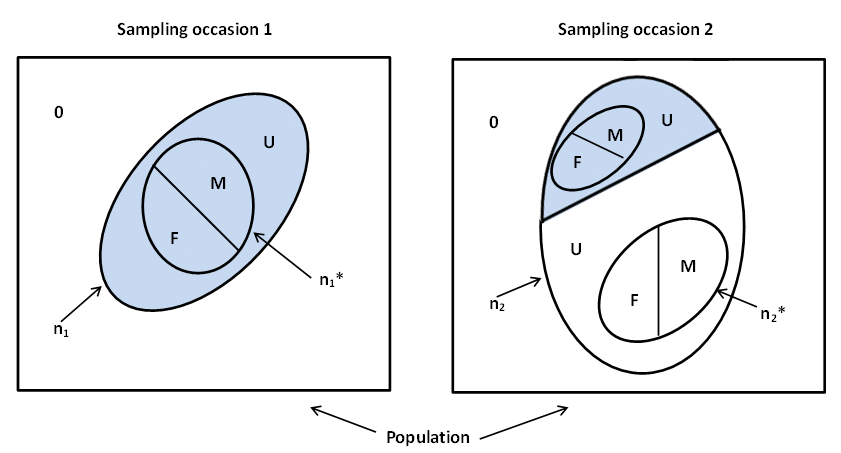
\includegraphics[scale=0.24]{CaptureRecaptureFig1.png}
    \label{fig:PSTSCRE}
\end{figure}


\end{columns}

\end{frame}


%%%%%%%%%%%%%%%%%%%%%%%%%%%%%%%%%%%%%%%%%%%%%%%%%%%%%%%%%%%%%%%%%%%%%%%%%%%%%%%%%%%%%%

\begin{frame} \frametitle{Example - Model Selection }
\vspace{3pt}

\textbf{{\scriptsize  Model Notation} }
{\tiny 
\begin{itemize}
\item Let $k$ stands for category and $t$ stands for time
\vspace{3pt}
\item Capture probability $p$ depends on $k$ and $t$,  sampling fraction $\theta$ depends on $t$ and category proportion $\lambda$ depends on $k$
\vspace{3pt}
\item For Example, 
\vspace{3pt}
\begin{itemize}
{\tiny 
\item $p_{k*t}$ implies that capture-probability varies by category  and time
\vspace{4pt}
\item $p_{t}$ implies capture-probabilities vary by time but not by category
\vspace{1pt}
\item $p_{.}$ implies capture-predictabilities do not vary by category or by time
}
\end{itemize}
\end{itemize}
}

%\begin{itemize}
%\item {\scriptsize  Following models have been considered for the model selection }
%\end{itemize}
%{\tiny
%\centering 
%\begin{tabular}{ l l } 
% $( p_{k*t},\theta_{t},\lambda_{k})$ & model with no restrictions \\ \vspace{2pt}
% $( p_{k*t},\theta_{t},\lambda_{.})$  & Category proportions are equal ($\lambda_{M} = \lambda_{F} = 0.5$)\\\vspace{2pt}
%$( p_{k},\theta_{t},\lambda_{k})$ &  Capture Probability does not vary by time ($p_{1M} = p_{2M}$  and $p_{1F} = p_{2F}$)\\\vspace{2pt}
% $( p_{.},\theta_{t},\lambda_{k})$  & All capture probabilities are equal ($p_{1M} = p_{1F} = p_{2M} = p_{2F}$)\\\vspace{2pt}
% $( p_{k*t},\theta_{.},\lambda_{k})$  & Equal sampling proportions ($\theta_{1} = \theta_{2}$)\\\vspace{2pt}
% $( p_{k*t},\theta_{t},\lambda_{k})$  & Capture Probabilities does not vary by time and Category proportions are equal\\\vspace{2pt}
% &\quad ($p_{1M} = p_{2M}$  and $p_{1F} = p_{2F}$ and \lambda_{M} = \lambda_{F} = 0.5$ )\\
% $( p_{.},\theta_{.},\lambda_{.})$  & Equal capture probabilities and equal sampling proportions and equal category proportions\\\vspace{2pt}
%& \quad($p_{1M} = p_{1F} = p_{2M} = p_{2F}$ and $\theta_{1} = \theta_{2}$ and $\lambda_{M} = \lambda_{F} = 0.5$)
%\end{tabular}
%
%}
%\begin{table}
%{\tiny 
%\centering 
%\begin{tabular}{|l|c|r|c|c|r|r|}
%\hline
%model & No: of Parameters & $max\left\lbrace ln(L)\right\rbrace$ &$\hat{N}$  &$s.e.(\hat{N}$) & $AICc$ \qquad  &$\Delta AICc$ \quad\\ \hline
% $( p_{k*t},\theta_{t},\lambda_{k})$ & 8    &      30.57& 205505& 26139&    77.16 &     0.00\\ \hline
%$( p_{k*t},\theta_{t},\lambda_{.})$ & 7    &      33.95& 208129& 24389&    81.92 &     4.76\\ \hline
%$( p_{k},\theta_{t},\lambda_{k})$ & 6    &     813.37& 399362& 54672&  1638.74 &  1561.58\\ \hline
% $( p_{.},\theta_{t},\lambda_{k}$ & 5    &     819.58& 348598& 39933&  1649.16 &  1572.00\\ \hline
% $( p_{k},\theta_{t},\lambda_{.})$ & 5    &    5840.31& 399377& 54676& 11690.63 & 11613.47\\ \hline
% $( p_{.},\theta_{.},\lambda_{.})$ & 3    &    6673.99& 348592& 39932& 13353.97 & 13276.81\\ \hline
%\end{tabular}
%}
%\end{table}

\begin{table}
{\tiny 
\centering 
\begin{tabular}{|l|c|r|r|r|r|r|}
\hline 
model & np & $max\left\lbrace ln(L)\right\rbrace$ &$\hat{N}$ (in $ 10^{3}$)  &$s.e.(\hat{N}$) (in $ 10^{3}$) & $AICc$ \qquad  &$\Delta AICc$ \quad\\ \hline
 $( p_{k*t},\theta_{t},\lambda_{k})$ & 8    &      30.57& 205.5& 26.1&    77.1 &     0.0\\ \hline
$( p_{k*t},\theta_{t},\lambda_{.})$ & 7    &      33.95& 208.1& 24.3&    81.9 &     4.7\\ \hline
$( p_{k},\theta_{t},\lambda_{k})$ & 6    &     813.37& 399.3& 54.6&  1638.7 &  1561.5\\ \hline
 $( p_{.},\theta_{t},\lambda_{k}$ & 5    &     819.58& 348.5& 39.9&  1649.1 &  1572.0\\ \hline
 $( p_{k},\theta_{t},\lambda_{.})$ & 5    &    5840.31& 399.3& 54.6& 11690.6 & 11613.4\\ \hline
 $( p_{.},\theta_{.},\lambda_{.})$ & 3    &    6673.99& 348.5& 39.9& 13353.9 & 13276.8\\ \hline
\end{tabular}
}
\end{table}

\end{frame}

%%%%%%%%%%%%%%%%%%%%%%%%%%%%%%%%%%%%%%%%%%%%%%%%%%%%%%%%%%%%%%%%%%%%%%%%%%%%%%%%%%%%%%
\begin{frame} \frametitle{Example}
\textbf{{\footnotesize Parameter Estimation }}
\begin{itemize}
\item {\scriptsize Parameter estimation in partial stratified two-sample capture-recapture model and  simple Lincoln-Petersen estimate for  population size ($\hat{N}_{LP}$)}
\end{itemize}
{\tiny
\begin{table}
\centering
\begin{tabular}{|l|r|r|r|}
\hline
Parameter & MLE\qquad \qquad & S.E. of the MLE  &  S.E.  $(p_{k*t},\theta_{k} \lambda{.}^{{\tiny MLE}} )$ \\ \hline
$p_{1M}$ 	& 7.58 $\times 10^{-2}$ 	 & 1.50 $\times 10^{-2}$  &  9.43 $\times 10^{-3}$ \\ \hline
$p_{1F}$ 	& 1.15 $\times 10^{-2}$   	 & 0.20 $\times 10^{-2}$  &  1.04 $\times 10^{-3}$ \\ \hline
$p_{2M}$ 	& 0.78 $\times 10^{-2}$    	 & 0.12 $\times 10^{-2}$  &  1.04 $\times 10^{-3}$ \\ \hline
$p_{2F}$ 	& 2.09 $\times 10^{-2}$		 & 0.36  $\times 10^{-2}$ &  2.82 $\times 10^{-3}$ \\ \hline
$\lambda_{M}$ & 3.29 $\times 10^{-1}$    & 6.05 $\times 10^{-2}$  &   0 \\ \hline
$\lambda_{F}$ & 6.70 $\times 10^{-1}$    & 6.05 $\times 10^{-2}$  &  0 \\ \hline
$\theta_{1}$  & 9.93 $\times 10^{-1}$    & 0.94  $\times 10^{-3}$ &  9.48$\times 10^{-3}$ \\ \hline
$\theta_{2}$  & 0.82 $\times 10^{-1}$    & 4.76  $\times 10^{-3}$  & 4.76 $\times 10^{-3}$ \\ \hline
$N$     & 2055.05 $\times 10^{2}$ \qquad     	 &   261.38 $\times 10^{2}$  \qquad    &  254.22   $\times 10^{2}$  \qquad  \\ \hline
$N_{M}$ &  677.84  $\times 10^{2}$ \qquad    	 &   133.91 $\times 10^{2}$  \qquad    &   83.85  $\times 10^{2}$  \qquad  \\ \hline
$N_{F}$ & 1377.21  $\times 10^{2}$  \qquad     &   237.29 $\times 10^{2}$   \qquad     &  170.36   $\times 10^{2}$  \qquad  \\ \hline \hline
$\hat{N}_{LP}$ & 3117.64  $\times 10^{2}$ & 347.17 $\times 10^{2}$  & \\ \hline

\end{tabular}
\end{table}
}
%{\tiny
%\begin{table}
%\centering
%\begin{tabular}{|l|r|r|r|}
%\hline
%Parameter & MLE\qquad \qquad & S.E. of the MLE  &  S.E.  $(p_{k*t},\theta_{k} \lambda{.}^{{\tiny MLE}} )$ \\ \hline
%$p_{1M}$ 	& 7.58 $\times 10^{-2}$ 	 & 1.50 $\times 10^{-2}$  &  9.43 $\times 10^{-3}$ \\ \hline
%$p_{1F}$ 	& 1.15 $\times 10^{-2}$   	 & 0.20 $\times 10^{-2}$  &  1.04 $\times 10^{-3}$ \\ \hline
%$p_{2M}$ 	& 0.78 $\times 10^{-2}$    	 & 0.12 $\times 10^{-2}$  &  1.04 $\times 10^{-3}$ \\ \hline
%$p_{2F}$ 	& 2.09 $\times 10^{-2}$		 & 0.36  $\times 10^{-2}$ &  2.82 $\times 10^{-3}$ \\ \hline
%$\lambda_{M}$ & 3.29 $\times 10^{-1}$    & 6.05 $\times 10^{-2}$  &   0 \\ \hline
%$\lambda_{F}$ & 6.70 $\times 10^{-1}$    & 6.05 $\times 10^{-2}$  &  0 \\ \hline
%$\theta_{1}$  & 9.93 $\times 10^{-1}$    & 0.94  $\times 10^{-3}$ &  9.48$\times 10^{-3}$ \\ \hline
%$\theta_{2}$  & 0.82 $\times 10^{-1}$    & 4.76  $\times 10^{-3}$  & 4.76 $\times 10^{-3}$ \\ \hline
%$N$     & 2055.05 $\times 10^{2}$ \qquad     	 &   261.38 $\times 10^{2}$  \qquad    &  254.22   $\times 10^{2}$  \qquad  \\ \hline
%$N_{M}$ &  677.84  $\times 10^{2}$ \qquad    	 &   133.91 $\times 10^{2}$  \qquad    &   83.85  $\times 10^{2}$  \qquad  \\ \hline
%$N_{F}$ & 1377.21  $\times 10^{2}$  \qquad     &   237.29 $\times 10^{2}$   \qquad     &  170.36   $\times 10^{2}$  \qquad  \\ \hline \hline
%$\hat{N}_{LP}$ & 3117.64  $\times 10^{2}$ & 347.17 $\times 10^{2}$  & \\ \hline
%
%\end{tabular}
%\end{table}
%}

\begin{itemize}
\item {\tiny Last column of the table is the estimates when the sex ratio is fixed at MLE}

\end{itemize}
\end{frame}


%%%%%%%%%%%%%%%%%%%%%%%%%%%%%%%%%%%%%%%%%%%%%%%%%%%%%%%%%%%%%%%%%%%%%%%%%%%%%%%%%%%%%%
%%%%%%%%%%%%%%%%%%%%%%%%%%%%%%%%%%%%%%%%%%%%%%%%%%%%%%%%%%%%%%%%%%%%%%%%%%%%%%%%%%%%%%
\begin{frame} \frametitle{Example}
\textbf{{\scriptsize Optimal Allocation of effort }}
\begin{itemize}
\item  {\scriptsize Use MLE's of $N$, $\lambda_{M}$, $r_{1}$, and $r_{2}$ (ratios of male to female at time 1 and 2)  as guestimates}
\item {\scriptsize  Considered $c_{1} =2 $, $c_{2} =c_{1}/2$, $c_{1}^{*} = 4$, $c_{2}^{*} = c_{1}^{*}/2 = 4$, $C_{0} =40000$}
\end{itemize}
\hspace{1cm} {\tiny Optimal allocation}

{\tiny 
$\qquad \qquad \qquad  n_{1} = 8199 $
\vspace{2pt}

$\qquad \qquad \qquad n_{1}^{*} = 3003$ 
\vspace{2pt}

$\qquad \qquad \qquad n_{2} = 9511$
\vspace{2pt}

$\qquad \qquad \qquad n_{2}^{*} = 997 $

$\qquad \qquad \qquad SE(\hat{N}) = 15904 $
\vspace{2pt}
}
\begin{itemize}
\item  {{\scriptsize  Conditional Contour plot and Graph for $SE(\hat{N})$ }}
\end{itemize}
\begin{columns}
\column{0.45\textwidth}
\hspace{1cm}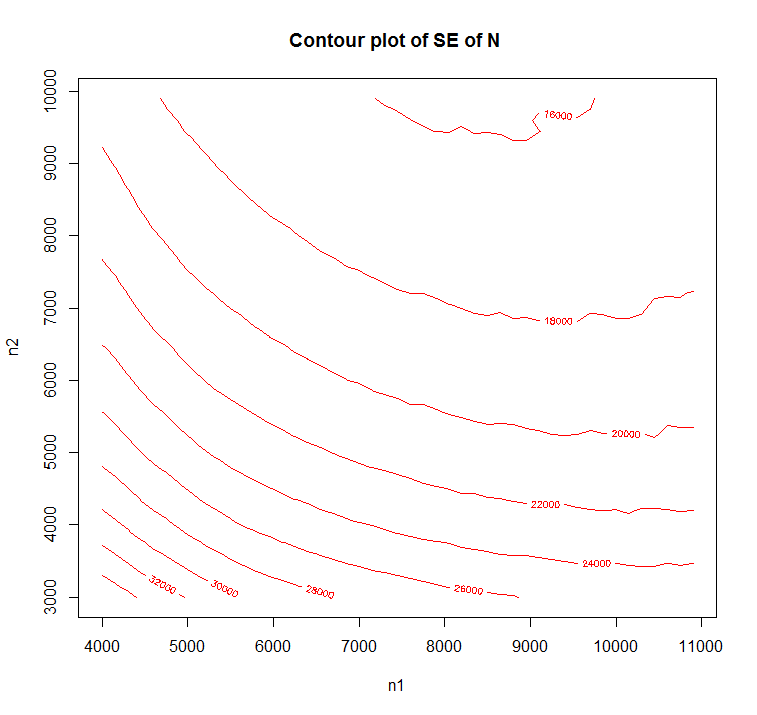
\includegraphics[scale=.14]{2014_05_19Contour_plot.png}
\column{0.45\textwidth}
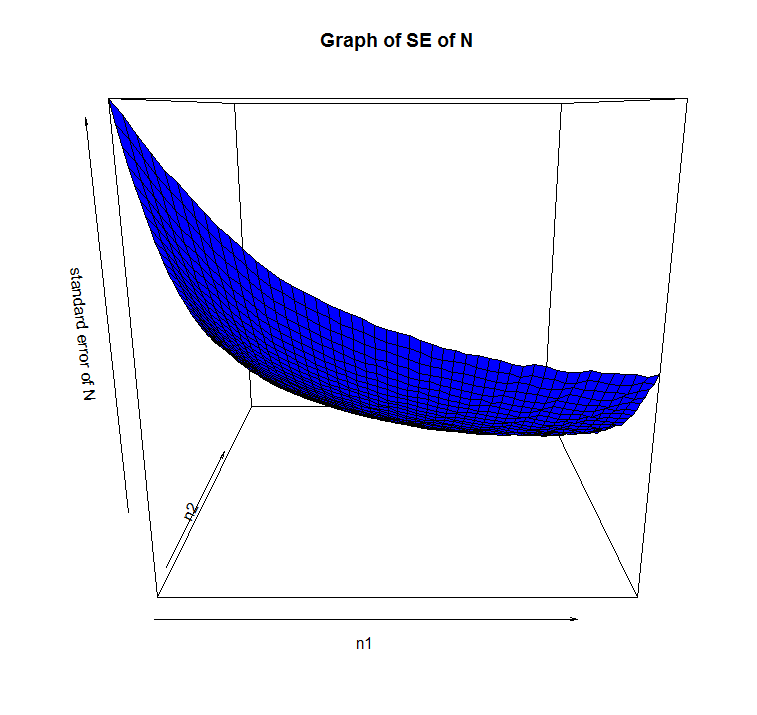
\includegraphics[scale=.14]{2014_05_19Graph_SE_N.png}
\end{columns}

\end{frame}

%%%%%%%%%%%%%%%%%%%%%%%%%%%%%%%%%%%%%%%%%%%%%%%%%%%%%%%%%%%%%%%%%%%%%%%%%%%%%%%%%%%%%%
%%%%%%%%%%%%%%%%%%%%%%%%%%%%%%%%%%%%%%%%%%%%%%%%%%%%%%%%%%%%%%%%%%%%%%%%%%%%%%%%%%%%%%
\section{Summary and Further Work}
%\begin{frame} \frametitle{Further Work}
%\textbf{{\scriptsize Development of Bayesian Solution}}
%
%{\scriptsize 
%\begin{itemize}
%\item Likelihood $L(N,p_{kt},\theta_{t},\lambda_{k}|\mathcal{D} )$  where $\mathcal{D}$ is data
%\vspace{6pt}
%
%\item The Prior Distributions
%\vspace{6pt}
%
%The improper prior distribution of Jeffrey, $\pi(N)= \frac{1}{N}$, is often used(King and Brooks,2001).
%and $Beta(1,1)$ prior for other parameters. 
%\vspace{12pt}
%
%\item The Gibbs Sampling Algorithm (use JAGS)
%\end{itemize}
%}
%\end{frame}

%%%%%%%%%%%%%%%%%%%%%%%%%%%%%%%%%%%%%%%%%%%%%%%%%%%%%%%%%%%%%%%%%%%%%%%%%%%%%%%%%%%%%%
\begin{frame} \frametitle{Summary}

\begin{itemize}
\item \textbf{{\scriptsize Problem}}
\begin{itemize}
{\scriptsize 
\item Capture heterogeneity is case bias in estimates in two-sample capture-recapture experiments 
\item Stratification is not possible for all captured animals in each occasion
\item Stratification is costly
}
\end{itemize}
\item \textbf{{\scriptsize Solution}}
\begin{itemize}
{\scriptsize 
\item A method developed using partial stratification 
\item Given the relative cost of sampling for a simple capture and for processing the sub-sample, optimal allocation of effort for a given cost can be determined.
\item Still the optimal allocation method has to be fine tuned.
\item Several methods used for finding the analytical solutions for MLE, but not plausible
}
\end{itemize}
\item \textbf{{\scriptsize  Future work}}
\begin{itemize}
{\scriptsize 
\item Bayesian solution
\begin{itemize}
\item {\scriptsize Why intersted in bayesian approach.}
\end{itemize}
\item Adding individual covariates
\item Extend the method for continuous covariates
}
\end{itemize}
\end{itemize}
\end{frame}


%%%%%%%%%%%%%%%%%%%%%%%%%%%%%%%%%%%%%%%%%%%%%%%%%%%%%%%%%%%%%%%%%%%%%%%%%%%%%%%%%%%%%%
\begin{frame}
\begin{center}
Sincere appreciation to my Supervisor Prof. Carl James Schwarz 
\vspace{50pt}

{\Large  THANK YOU.}
\end{center}
\end{frame}


\end{document}